\begin{frame}
\frametitle{A reasonable theory}

\begin{columns}
\column{0.35\textwidth}
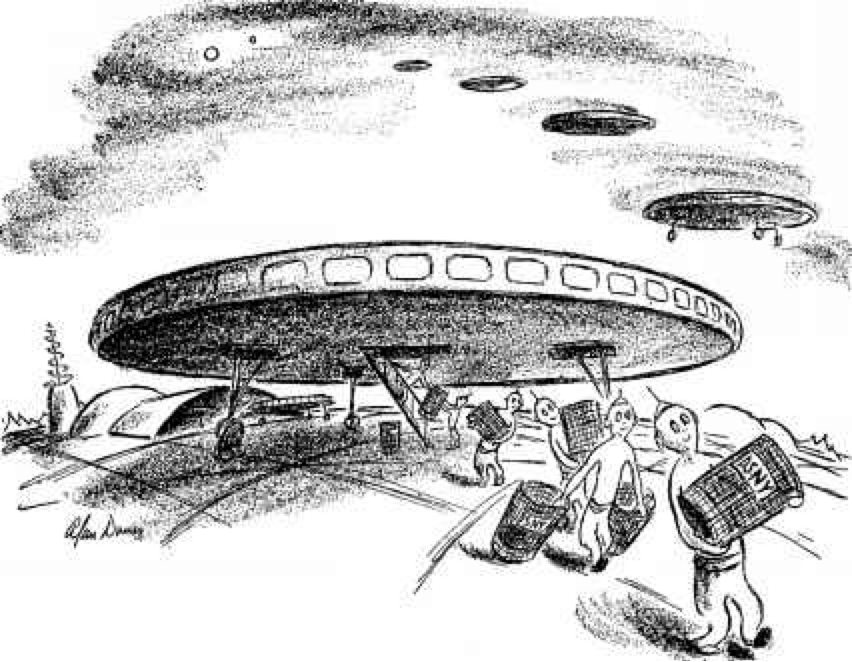
\includegraphics[scale=0.3]{aliens}
New Yorker cartoon by Alan Dunn in the New Yorker


 \column{0.5\textwidth}
%\begin{block}{}
In the Spring of 1950 the New York newspapers reported simultaneously the disappearance of public trash cans and numerous flying saucer observations. \vspace{0.5cm}

Fermi was at Los Alamos in the summer of 1950. One day, he was chatting to Edward Teller and Herbert York and Emil Konopinski told them of the Dunn cartoon. Fermi remarked wryly that Dunn's was a reasonable theory because it accounted for two distinct phenomena: the disappearance of trash cans and the reports of flying saucers. 
%\end{block}
\end{columns}
\end{frame}

\begin{frame}
\frametitle{Where is everybody?}

\begin{columns}
\column{0.35\textwidth}
\includegraphics[scale=0.3]{tellerfermi.jpeg}
Fermi and Teller in 1951


 \column{0.5\textwidth}
%\begin{block}{}

During lunch Fermi asked suddenly: "Where is everybody?" His lunch partners immediately understood that he was talking about aliens. York recalls that Fermi made a series of rapid calculations and concluded that we should have been visited long ago and many times over.

\vspace{0.5cm}

Although neither Fermi nor the others ever published any of these calculations, we can make a reasonable guess at his thought processes. He must first have made an estimate of the number of ETCs in the Galaxy, and this is something we can estimate ourselves. After all, the question "How many advanced communicating extraterrestrial civilizations are there in the Galaxy?" is a typical Fermi question!
\end{columns}
\end{frame}